\section{Claims}
In this thesis, we describe and analyze a way for a user to query an external machine-learning algorithm for the classification of a possible attack (figure~\ref{fig:eval-model}). More specifically, The machine-learning model has been trained beforehand and is described my model parameters. Both the privacy of the query and the model parameters are preserved trough multi-party computation; the type of machine-learning algorithm queried is known as well as the reductions used. As the execution of MPC-based algorithms is very expensive, we suggest outsourcing (in a cloud) it to a group of servers (in our case 3), but the protocols described can directly be used between the different parties without outsourcing, in any $n$-party setting. All the interactions between the cloud, the user and model owners(s) are done using secure connections (TCP), as well as the connections between the servers of the cloud.

\begin{figure}
    \centering
    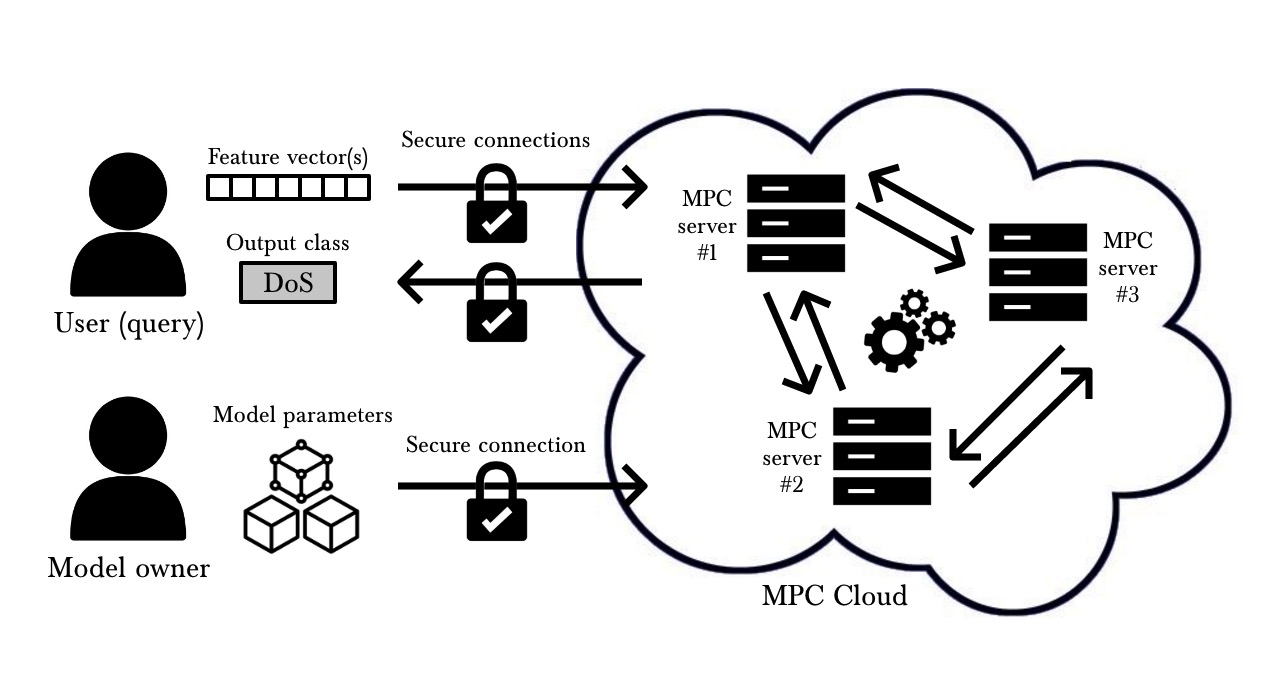
\includegraphics[width=.95\textwidth]{parts/chap-1/img-1/eval-model.jpg}
    \caption[Proposed setting]{Proposed setting for privacy-friendly machine-learning algorithms for intrusion detection systems.} 
    \label{fig:eval-model}
\end{figure}

We provide algorithmic solutions to the evaluation of support vector machines using secret sharing. Both linear as radial-based functions are implemented. To the best of our knowledge, this is the first time non-linear support vector machines are implemented under MPC security constraints. Due to the cost of MPC, the training of SVMs becomes very expensive. These algorithms are thus limited to evaluation against already trained models and thus the use of only one model owner. We showed that linear SVMs allow rapid evaluation of a query, especially when reduction methods are used. Non-linear SVMs are too slow, even with the reductions investigated.

We also provide algorithmic solutions to the nearest neighbors evaluation using the same secret sharing. We show that condensed nearest neighbors allow to make nearest neighbors practically feasible in the case of privacy-friendly intrusion detection systems.

Trade-offs that can be made to reduce the various costs of classical support vector machines and nearest neighbors, are investigated. Various reduction methods are pushed to their limits to see if they allow both of these algorithm to run in reasonable times to be used with multi-party computation. This comprises research in both the domains of machine-learning algorithms for intrusion detection systems and MPC-based machine-learning algorithms.

Furthermore, this thesis systematically compares the implementation of two different SVMs multi-class models: one-against-all and tree-based models. Up to now, they were alternatively used in the literature without systematic comparison. Tree-based models appear to be much faster without a loss of performance, both with linear as non-linear support vector machines.

We also investigate how feature size reduction methods such as PCA reduction or $\chi^2$ feature selection impact the classification performance and speed of the algorithm. To our knowledge, $\chi^2$ feature selection has never been applied before to nearest neighbors algorithms in the case of intrusion detection systems.

Next to investigating feature size reduction, we also investigate instance-set (or training set) size reduction: $k$-means and condensed nearest neighbors. To our knowledge, none of these algorithms have been applied to nearest neighbors in the case of intrusion detection systems. The condensed nearest neighbors allow to dramatically decrease the computation cost of the evaluation.

The two algorithms we present are practically usable in the proposed setting as they have limited computational, communication and round cost, for a totally satisfying classification accuracy.